\subsection{Direct Detection}

The DD constraints for the scalar and pseudoscalar mediator scenario are very different. While the scalar features an unsuppressed SI scattering cross section, the pseudoscalar cross section is highly suppressed at tree level such that the dominant contribution arises from loop graphs.

\subsubsection{Scalar}

We will generate DD constraints using the 2016 LUX~\citep{Akerib:2016vxi} and XENON1T~\citep{Aprile:2017iyp} data, via an effective operator approach using tools from \citep{DelNobile:2013sia}. The scattering of DM with nuclei will be dominated by the tree-level exchange of $S_1$ and $S_2$, resulting in a spin-independent scattering cross section. The only relevant nucleon operator is
\begin{align}
O_1^N = \bar{\chi} \chi \bar{N} N,  
\end{align}
and, by integrating out the mediators, we obtain a coefficient of \citep{Bell:2016ekl}
\begin{align}
c_N = m_N\frac{y_\chi \cos\theta\sin\theta}{v}\left(\frac{1}{M_{S_1}^2}-\frac{1}{M_{S_2}^2}\right) \left(f_{T_u}^N\epsilon_u + \epsilon_d\sum_{q=d,s} f_{T_q}^N + \frac{2}{9} f_{T_g} \frac{2 \epsilon_u+ \epsilon_d}{3} \right).
\label{eq:DDcoeff}
\end{align}

As there are contributions from exchange of the two scalars, with a relative negative sign, there is the possibility for destructive interference when the masses of $S_1$ and $S_2$ are comparable. 
%
In addition, depending on the choice of Yukawa structure, it is possible to have destructive interference between the up-type quarks and the down-type quarks in the nucleon. For the Type I and Type II Yukawa structure, the coefficients become
%
\small
\bea
c_N^{\text{type I}} &=&  m_N\frac{y_\chi \cos\theta\sin\theta}{v\tan\beta}\left(\frac{1}{M_{S_1}^2}-\frac{1}{M_{S_2}^2}\right) \left(\sum_{q=u,d,s} f_{T_q}^N  + \frac{2}{9} f_{T_g} \right),\\
c_N^{\text{type II}} &=&  m_N\frac{y_\chi \cos\theta\sin\theta}{v}\left(\frac{1}{M_{S_1}^2}-\frac{1}{M_{S_2}^2}\right) \left(f_{T_u}^N\cot\beta - \tan\beta\sum_{q=d,s} f_{T_q}^N + \frac{2}{9} f_{T_g} \frac{2\cot\beta-\tan\beta}{3} \right),
\label{scalarDD_typeII}
\eea
\normalsize
%
For the Type II scenario, we see that the presence of destructive $u$-$d$ interference is clearly visible in the right-hand bracket of \ref{scalarDD_typeII}. There is no such interference for Type I. If we adopt the values of $f_{T_i}$ obtained by~\citep{Gondolo:2004sc}, we find that a ratio of $\epsilon_u \sim - 1.6 \epsilon_d$ (corresponding to $\tan\beta=\sqrt{|\frac{\epsilon_d}{\epsilon_u}|}\sim 0.8$ in a Type II scenario) will result in exact cancellation of the DD signal.


In Figure~\ref{fig:SDD} we show the current DD exclusion from LUX \citep{Akerib:2016vxi} and XENON1T\citep{Aprile:2017iyp} together with the projections for XENON1T, XENONnT projections \citep{Aprile:2015uzo}.  We also show the sensitivity for a cross section equivalent to the ``neutrino floor" \citep{Billard:2013qya}.  We find that DD excludes significant parameter space, unless the scalar masses are approximately degenerate.  This can be seen in all 4 panels of Figure~\ref{fig:SDD} where we see a narrow allowed region near $M_{S_1} \sim M_{S_2}$, between excluded regions at higher and lower $M_{S_1}$ values.  
The excluded region in the upper LH plot (Type I) is somewhat larger than in the lower LH plot (Type II) lower due to the additional interference effect for the latter.
Increasing $\tan\beta$ weakens the constraints for Type I because $|\epsilon_d|=|\epsilon_u|=1/\tan\beta$ (upper right) and strengthens them for Type II because $|\epsilon_d|=|1/\epsilon_u|=\tan\beta$ (lower right).



%%%%%%%%%%%%%%%%%%%%%%%%%%%%%%%%%%%%%%%%%%%%%%%%%%%%%%%%%%%
\begin{figure}[ht]
\begin{center}
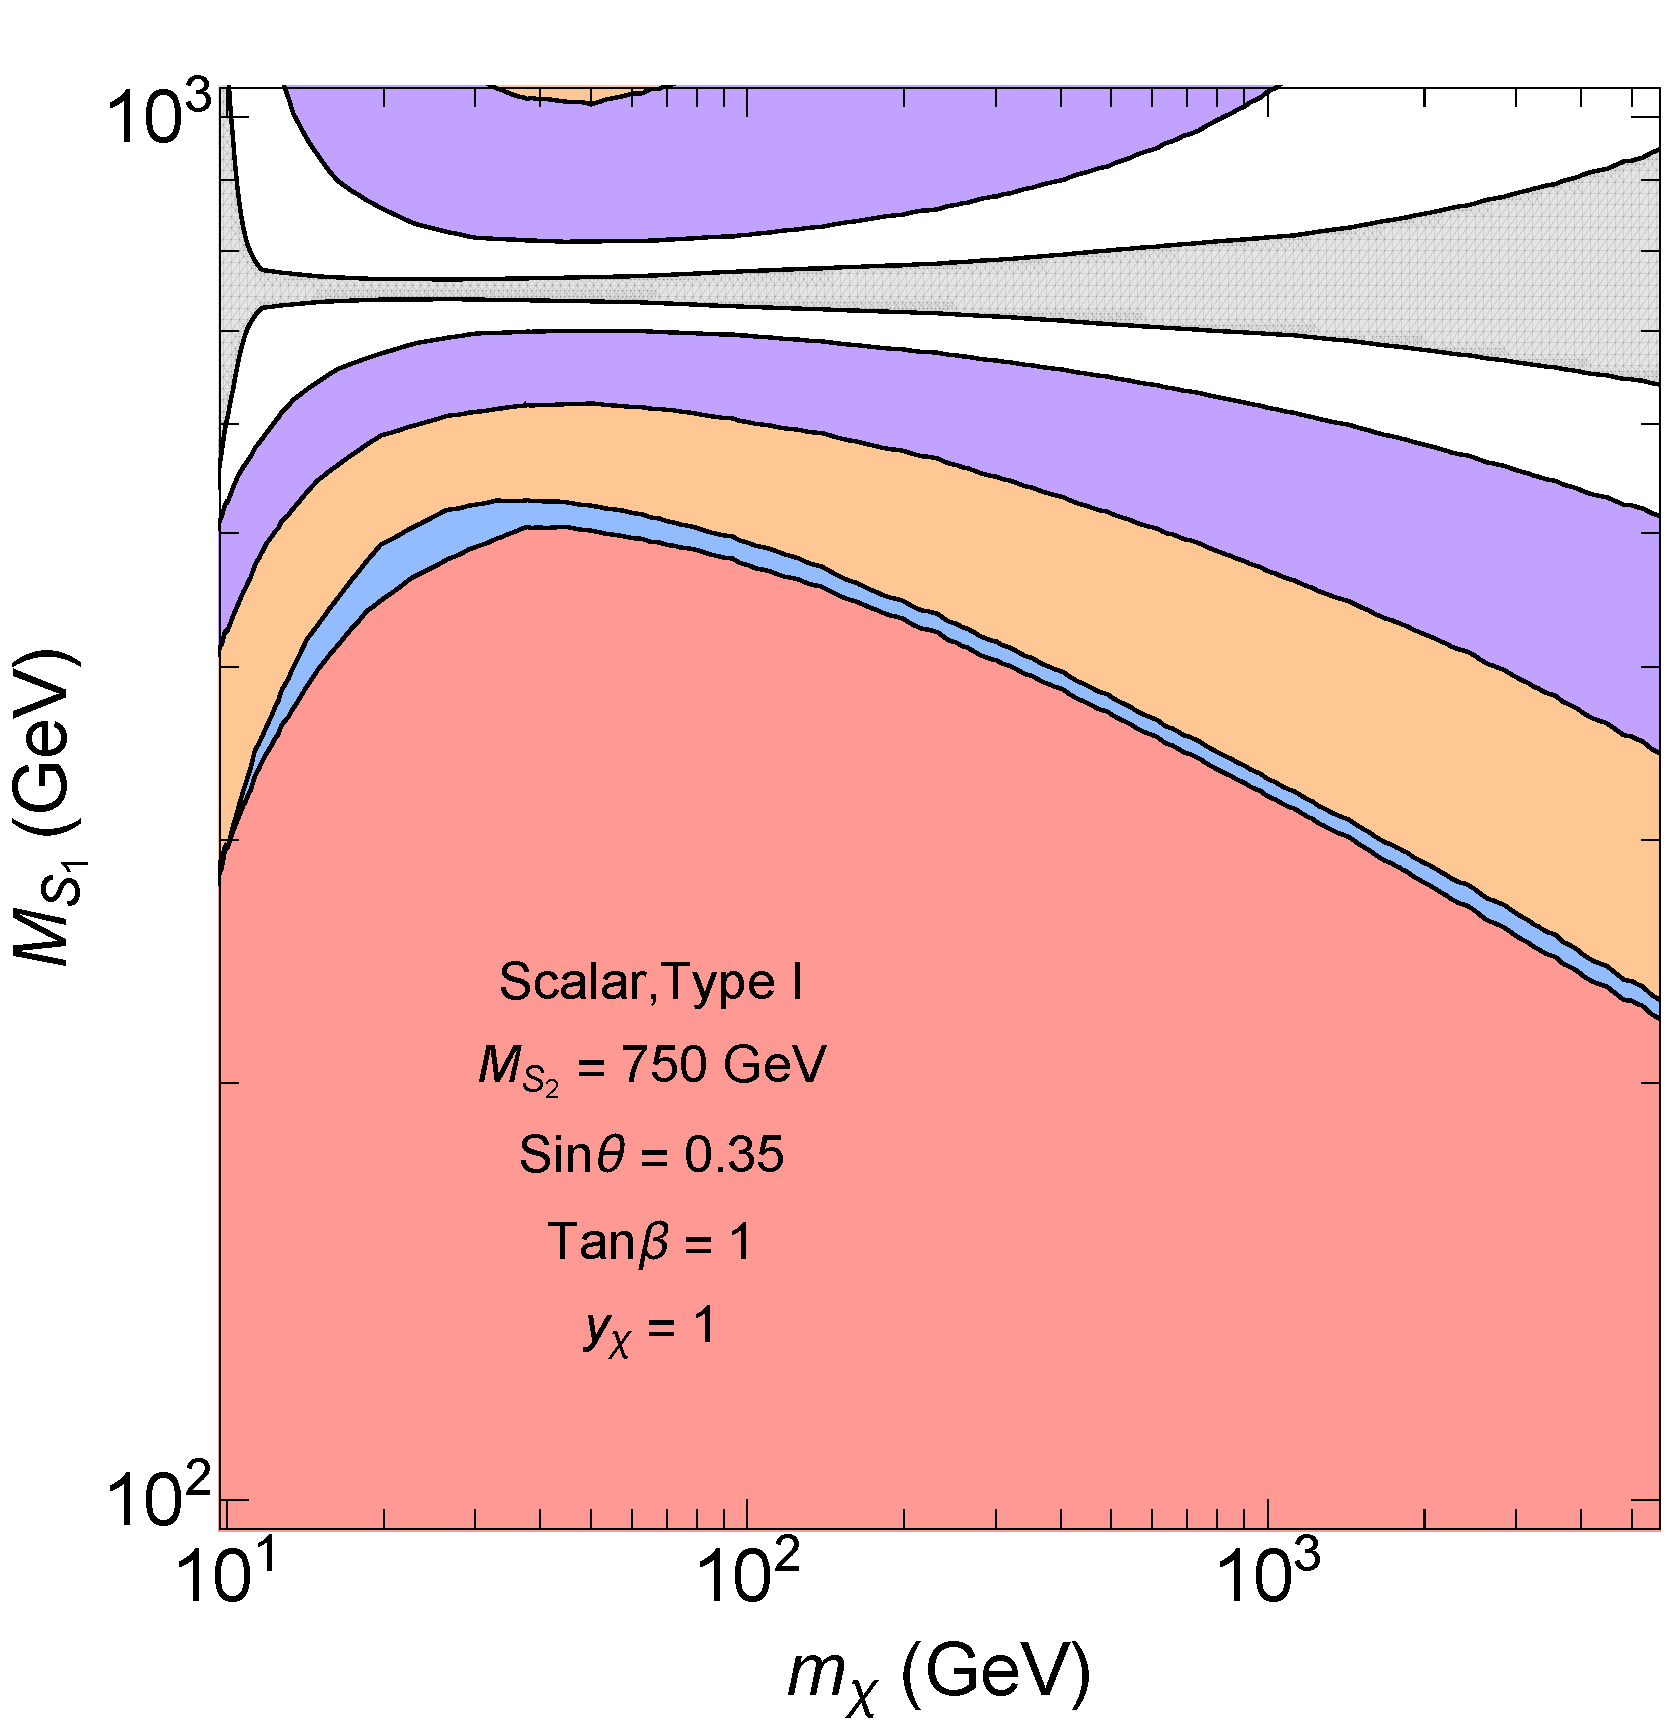
\includegraphics[width=0.49\textwidth]{texinputs/06_comparisons/figures/S_TI_TB1.pdf}
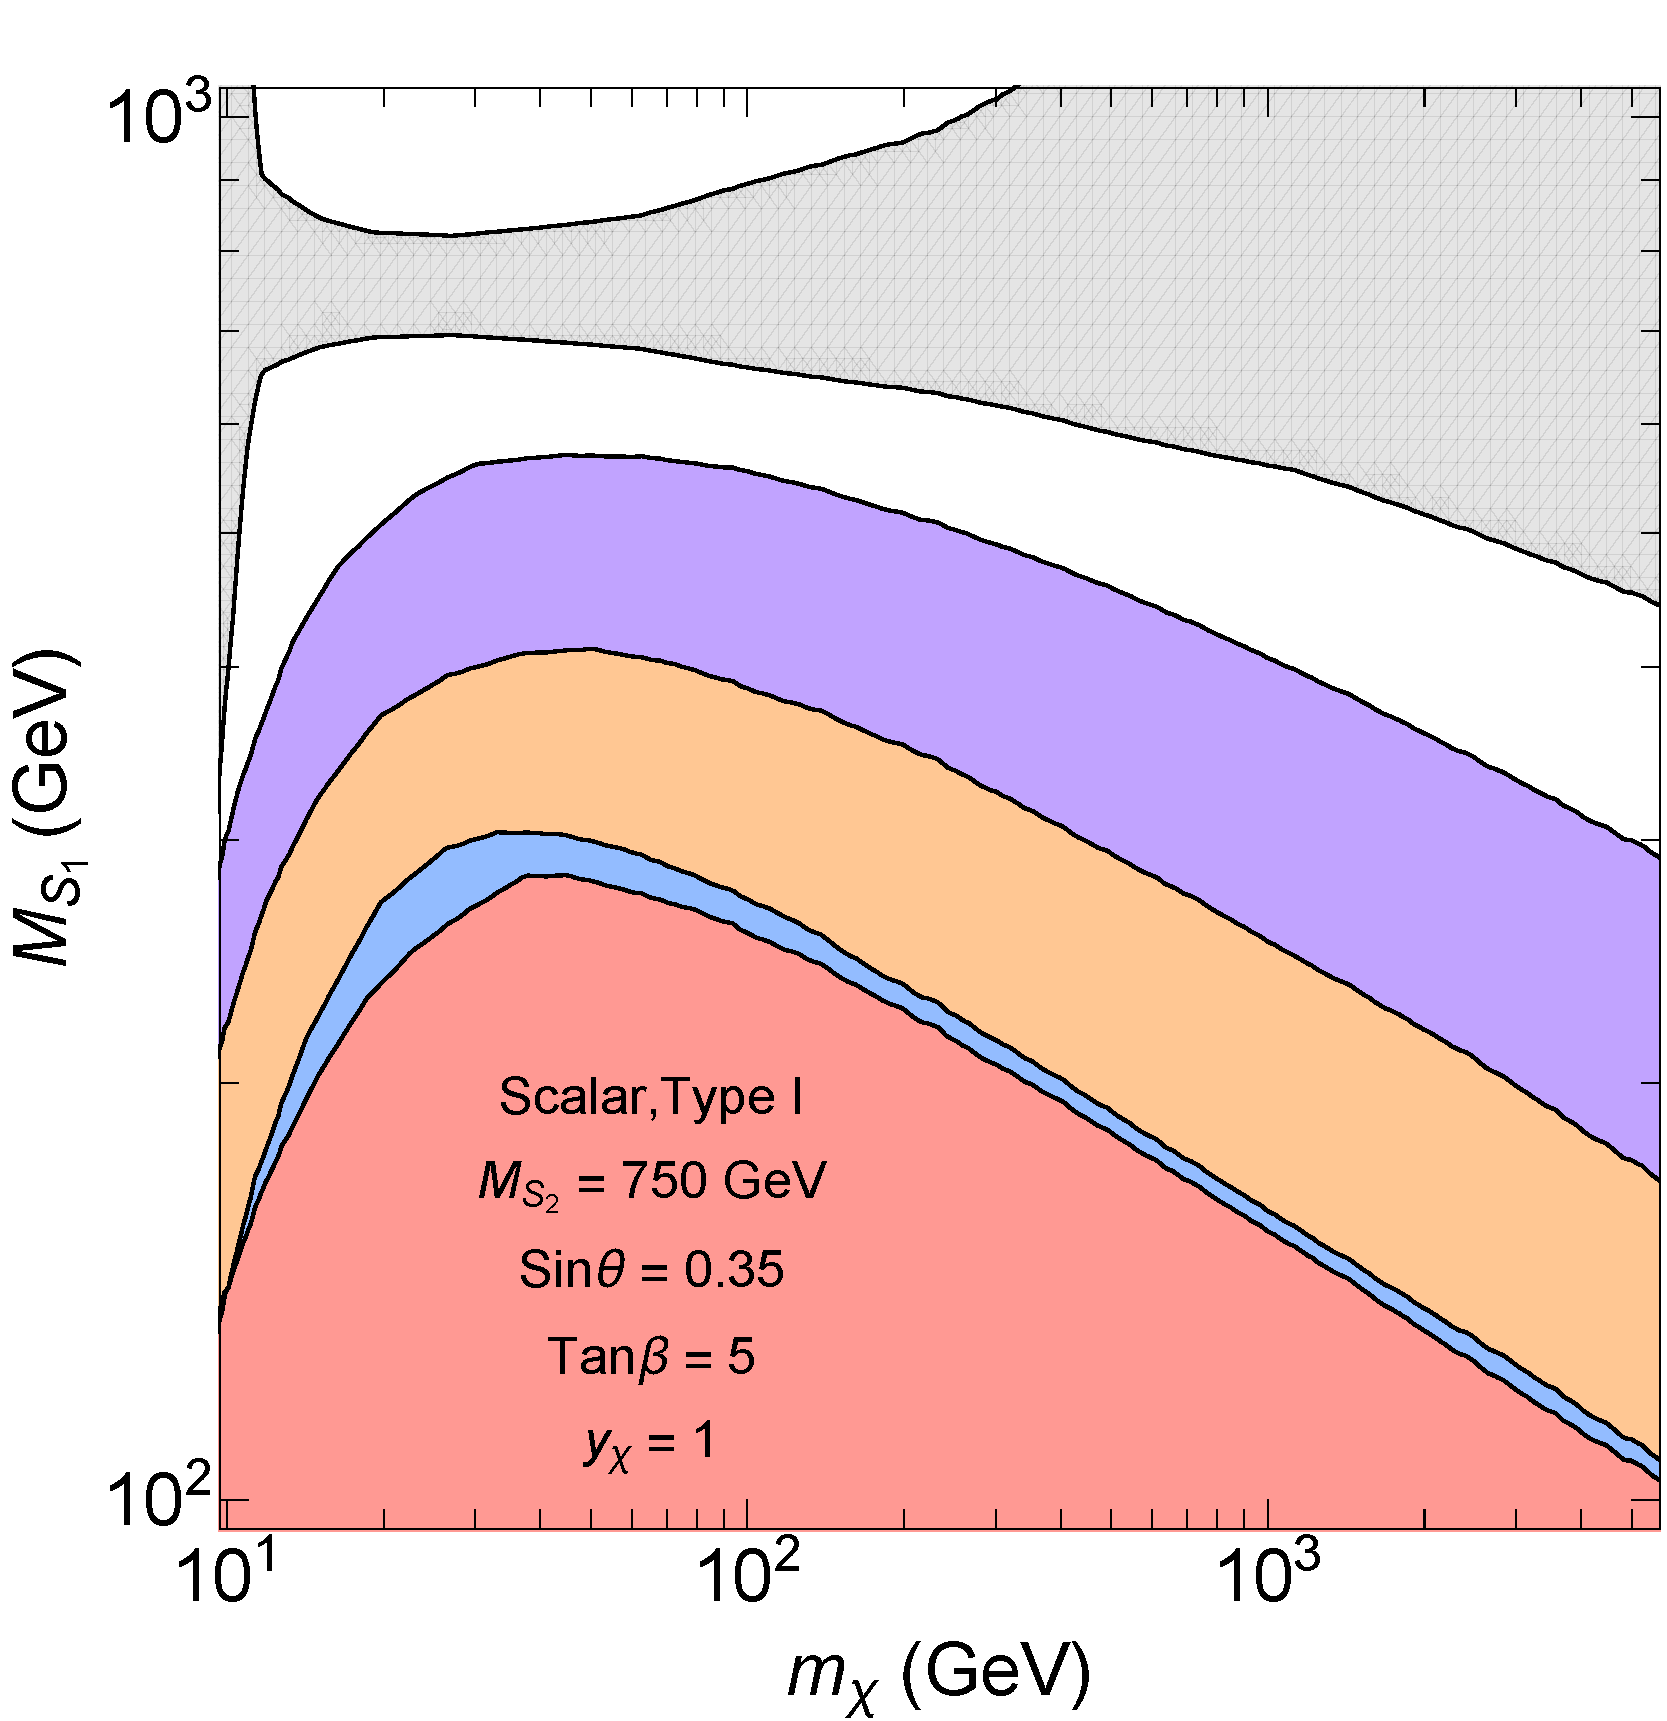
\includegraphics[width=0.49\textwidth]{texinputs/06_comparisons/figures/S_TI_TB5.pdf}\\
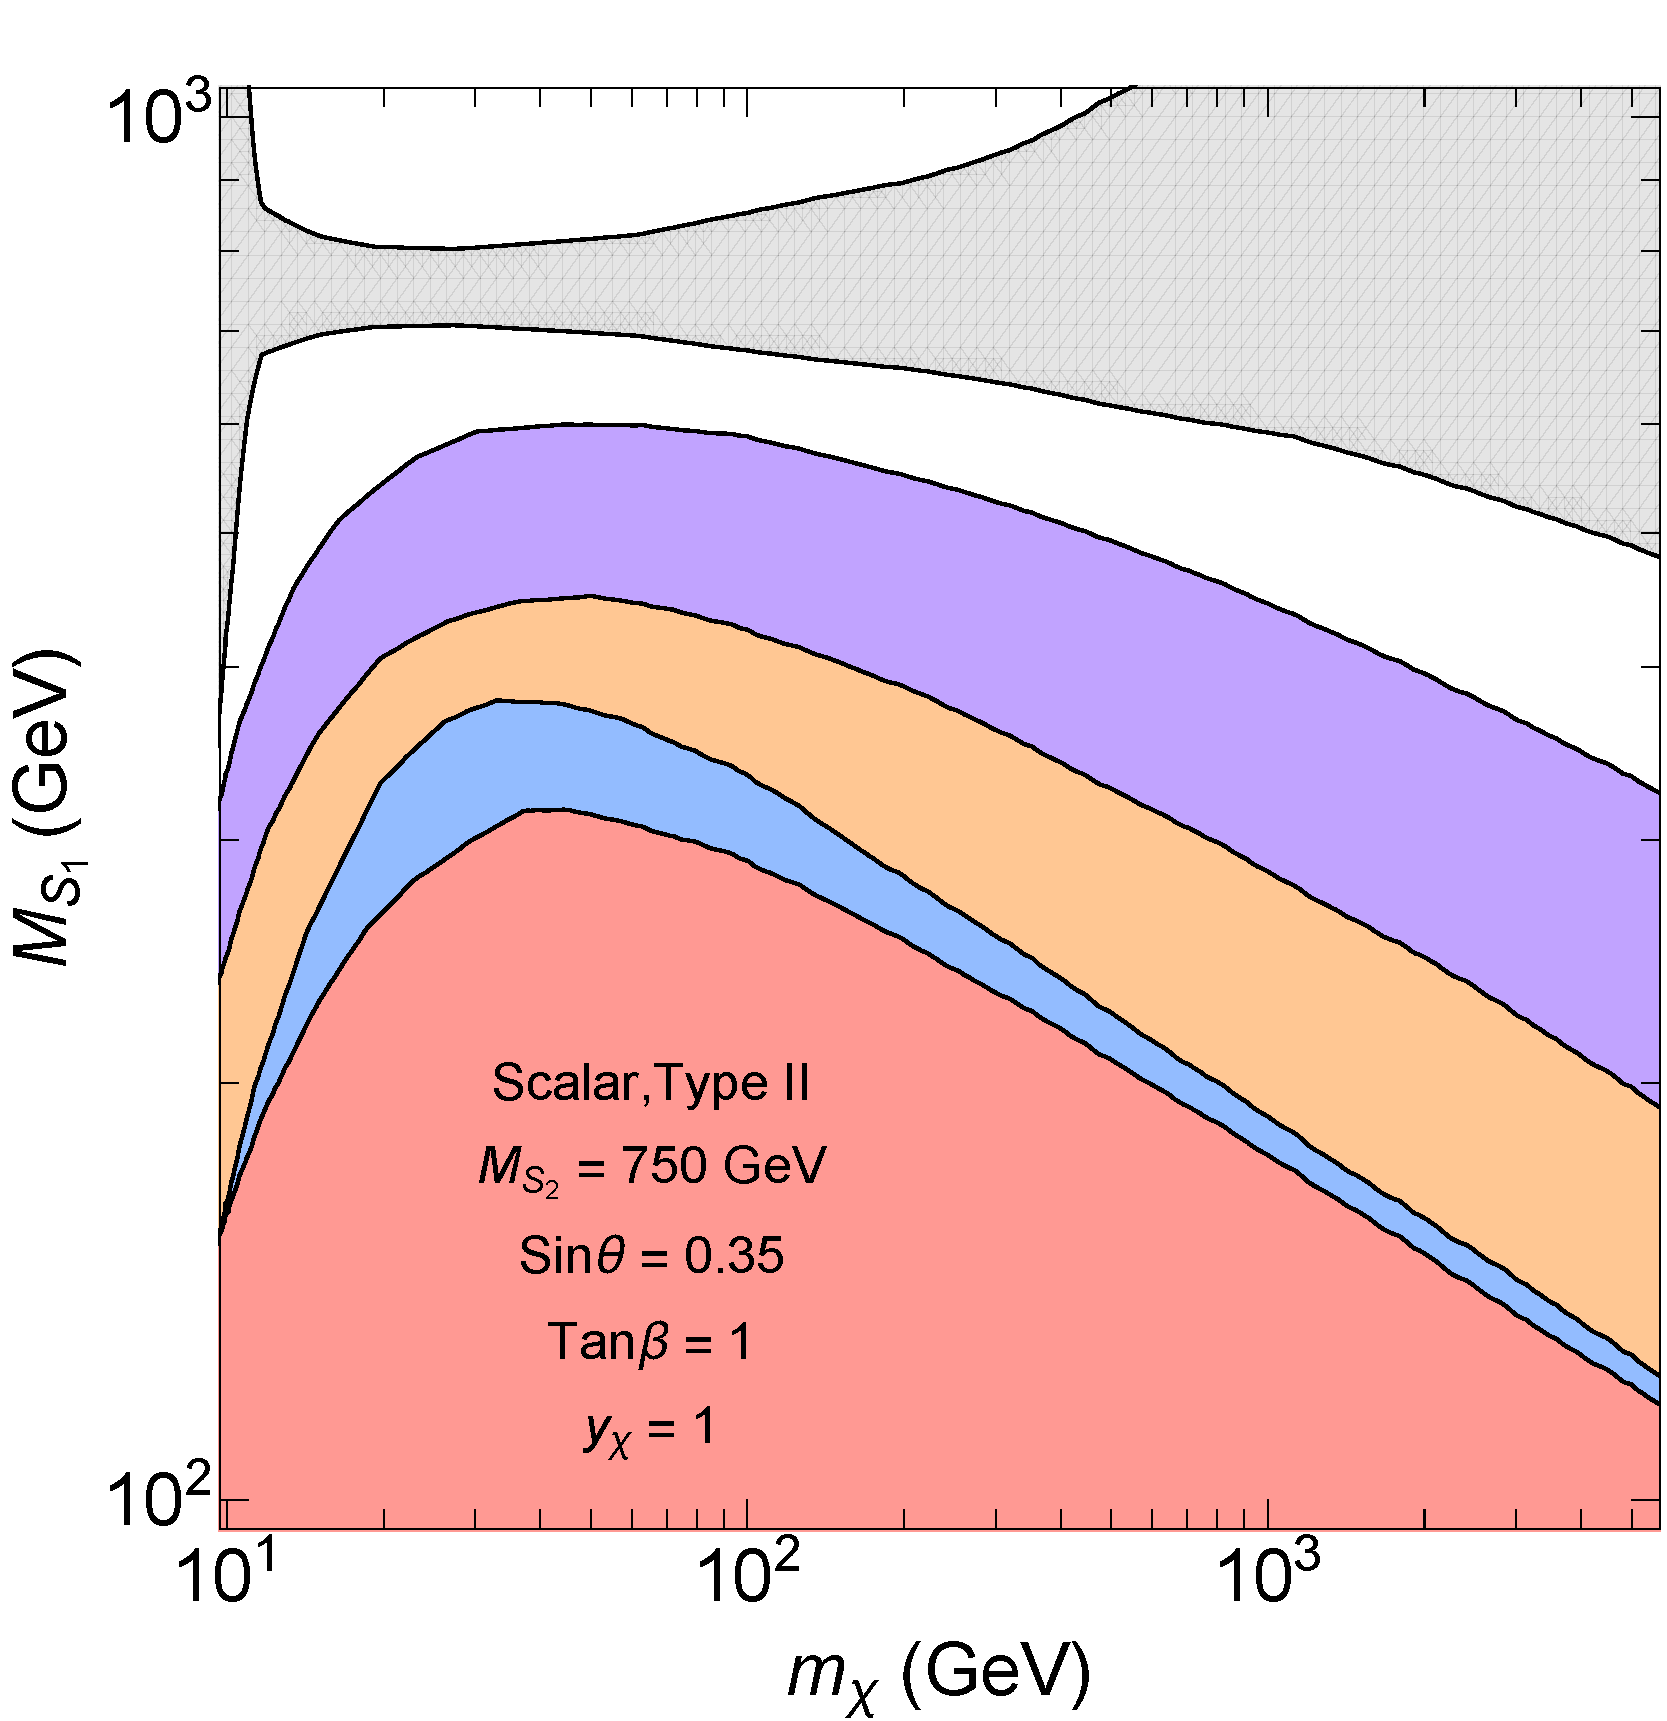
\includegraphics[width=0.49\textwidth]{texinputs/06_comparisons/figures/S_TII_TB1.pdf}
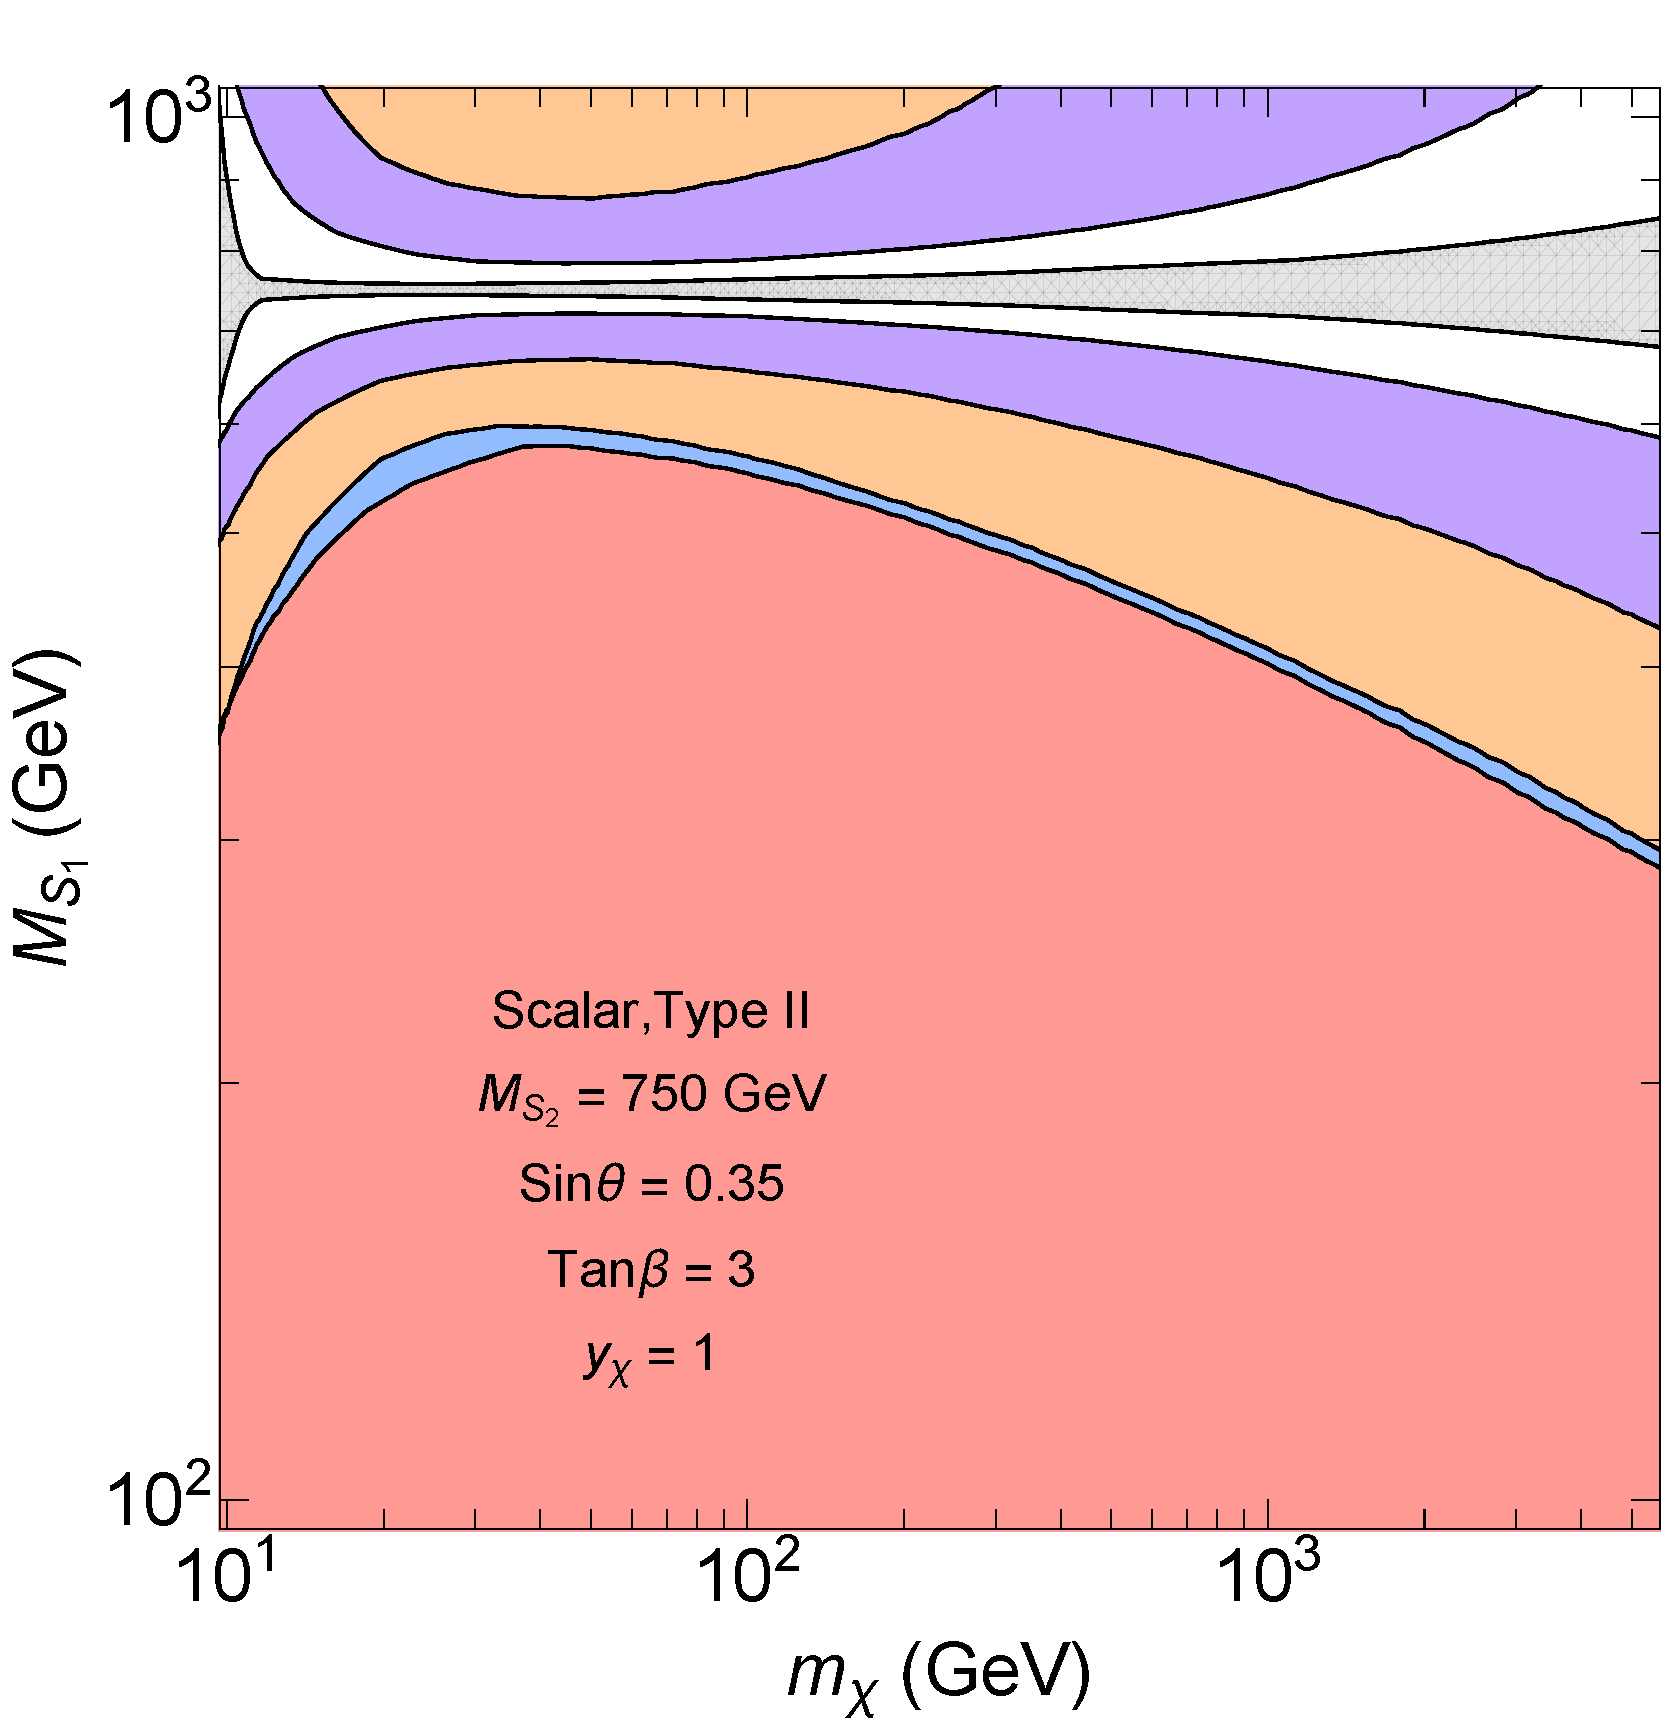
\includegraphics[width=0.49\textwidth]{texinputs/06_comparisons/figures/S_TII_TB3.pdf}
\caption{DD exclusion and projections for various experiments for the Scalar model. The various regions refer, in order, to LUX \citep{Akerib:2016vxi}, XENON1T\citep{Aprile:2017iyp}, XENON1T and XENONnT projections \citep{Aprile:2015uzo}, and neutrino background \citep{Billard:2013qya}. The mixing angle is set to $\sin\theta=0.35$, but results are equivalent also for $\cos\theta=0.35$, while $M_{S_2}=750\GeV$ in all the panels.} 
\label{fig:SDD}
\end{center}
\end{figure} 
%%%%%%%%%%%%%%%%%%%%%%%%%%%%%%%%%%%%%%%%%%%%%%%%%%%%%%%%%%%

\subsection{Pseudoscalar}

\begin{figure}[ht]
    \centering
    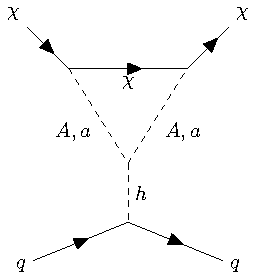
\includegraphics[width=0.3\textwidth]{texinputs/06_comparisons/figures/pseudoTriangle.pdf} \hspace{0.02\textwidth}
    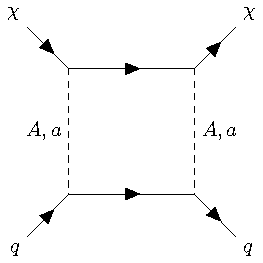
\includegraphics[width=0.3\textwidth]{texinputs/06_comparisons/figures/pseudoBox.pdf} \hspace{0.02\textwidth}
    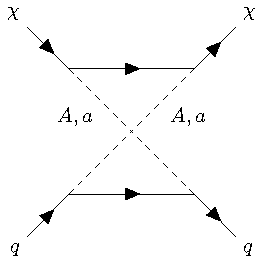
\includegraphics[width=0.3\textwidth]{texinputs/06_comparisons/figures/pseudoBox2.pdf} 
    \caption{Spin-independent DM-nucleon scattering arises from the loop exchange of the mixing pseudoscalar mediators. Left panel: triangle diagrams. Central and right panel: box diagrams.}
    \label{fig:feynDDPS}
\end{figure}



At tree level, the spin-independent scattering cross section is absent. The spin-independent cross section is non-zero, but highly suppressed due to a dependence on $q_{tr}^4$. At loop level, however, a spin-independent cross section is generated through the diagrams in Fig. \ref{fig:feynDDPS}. 
The triangle diagrams in the left panel of Fig. \ref{fig:feynDDPS} are proportional to $m_q$ while the box diagrams in the central and right panels of Fig. \ref{fig:feynDDPS} are proportional to $m_q^3$, thus the box diagrams are sub-leading as found in \citep{Ipek:2014gua} (except for Type II with $\tan\beta\gtrsim50$).
The triangle diagram does not depend on the Yukawa sector of the 2HDM. ** cite our paper in preparation**

Similarly as in the scalar model, in the PS model the mixing arises through a term $i b_P P \Phi_1^\dagger \Phi_2 +h.c.$. The resulting mixing angle is defined by

\begin{equation}
    b_P = -\frac{(M_A^2-M_a^2)\sin2\theta}{2v}
\end{equation}

%*** define $\sin 2\theta$  in terms of $\mu_{12s}$ somewhere ***\\
%*** also define $\lambda_{34-5}$ ***\\
%*** remove discussion of why  \citep{Ipek:2014gua} is wrong ***


The low energy effective operator generated at 1 loop is%in the approximation $M_{A}\gg M_{a}$ (in which case one considers only the diagram with two $a$'s appearing in the loop) is
\begin{eqnarray}
\mathcal{L}_{eff} &=& - \frac{y_\chi^2 m_q m_\chi}{16\pi^2 m_h^2 v^2}     G\left(\frac{m_\chi^2}{M_{A}^2},\frac{m_\chi^2}{M_{a}^2},\frac{m_h^2}{m_\chi^2},\theta\right) \bar{\chi}\chi\bar{q}q\label{eq:loopps}\\
G\left(x,y,z,\theta\right) &=& F_1(x)\sin^2\theta\hat{\mu}_{AAh}+F_1(y)\cos^2\theta\hat{\mu}_{aah}+F_2(x,y)\sin2\theta\hat{\mu}_{Aah}\label{eq:f2}\\
F_1(x) &=& \int_0^1 dz \frac{x (1-z) z}{x z^2-z+1} = \frac{(6 x-2) \log \left(\frac{\sqrt{1-4 x}+1}{2 \sqrt{x}}\right)+\sqrt{1-4 x} ((x-1) \log (x)-2 x)}{2 \sqrt{1-4 x} x}\label{eq:f1}\\
F_2\left(x,y\right) &=& \int_0^1 dz \frac{x y z \log \left(\frac{x y z^2-y z+y}{x y z^2-x z+x}\right)}{y-x} \nonumber\\
= \frac{1}{4xy(x-y)} &\bigg(&x^2 ((2 y-1) \log (y)-2 y)+x^2 \sqrt{1-4 y} \left(\log (4 y)-2 \log \left(\sqrt{1-4 y}+1\right)\right) \\
&-&2 x y^2 (\log (x)-1)+y^2 \log (x)+\sqrt{1-4 x} y^2\left(2 \log \left(\sqrt{1-4 x}+1\right)-\log (4 x)\right) \bigg)
%&=&\frac{x^2 ((2 y-1) \log (y)-2 y)+x^2 \sqrt{1-4 y} \left(\log (4 y)-2 \log \left(\sqrt{1-4 y}+1\right)\right)-2 x y^2 (\log (x)-1)+y^2 \log (x)+\sqrt{1-4 x} y^2\left(2 \log \left(\sqrt{1-4 x}+1\right)-\log (4 x)\right)}{4 x y (x-y)}\label{eq:f3}
\end{eqnarray}
%Our result differs from the one found in \citep{Ipek:2014gua} because of two reasons. First, we find that the amplitude contains an additional $\cos^2\theta$ factor, coming from the $\bar{\chi}\chi a$ yukawa couplings, on the top of the $\sin^2 2\theta$ factor coming from the cubic scalar vertex $aah$. Second, we find that the cubic scalar vertex $aah$ receives contributions not only from the portal term $\frac{1}{2}(i\mu_{hHP} \Phi_1^\dagger \Phi_2 P + h.c.)$, but also from the 2HDM terms proportional to $\lambda_{3},\lambda_{4}$ and $\lambda_{5}$, as it is manifest in Eq. \ref{eq:mu22h} \comm{add $\lambda_{P,1,2}$}. Depending on the point of the parameter space, these differences can be significant. To reduce the number of free parameters, we will fix $(\hat{\lambda}_3+\hat{\lambda}_4-\hat{\lambda}_5)v^2=\lambda_{34-5}v^2=m_h^2$ through all the section, as a benchmark point.

\begin{figure}[ht]
\begin{center}
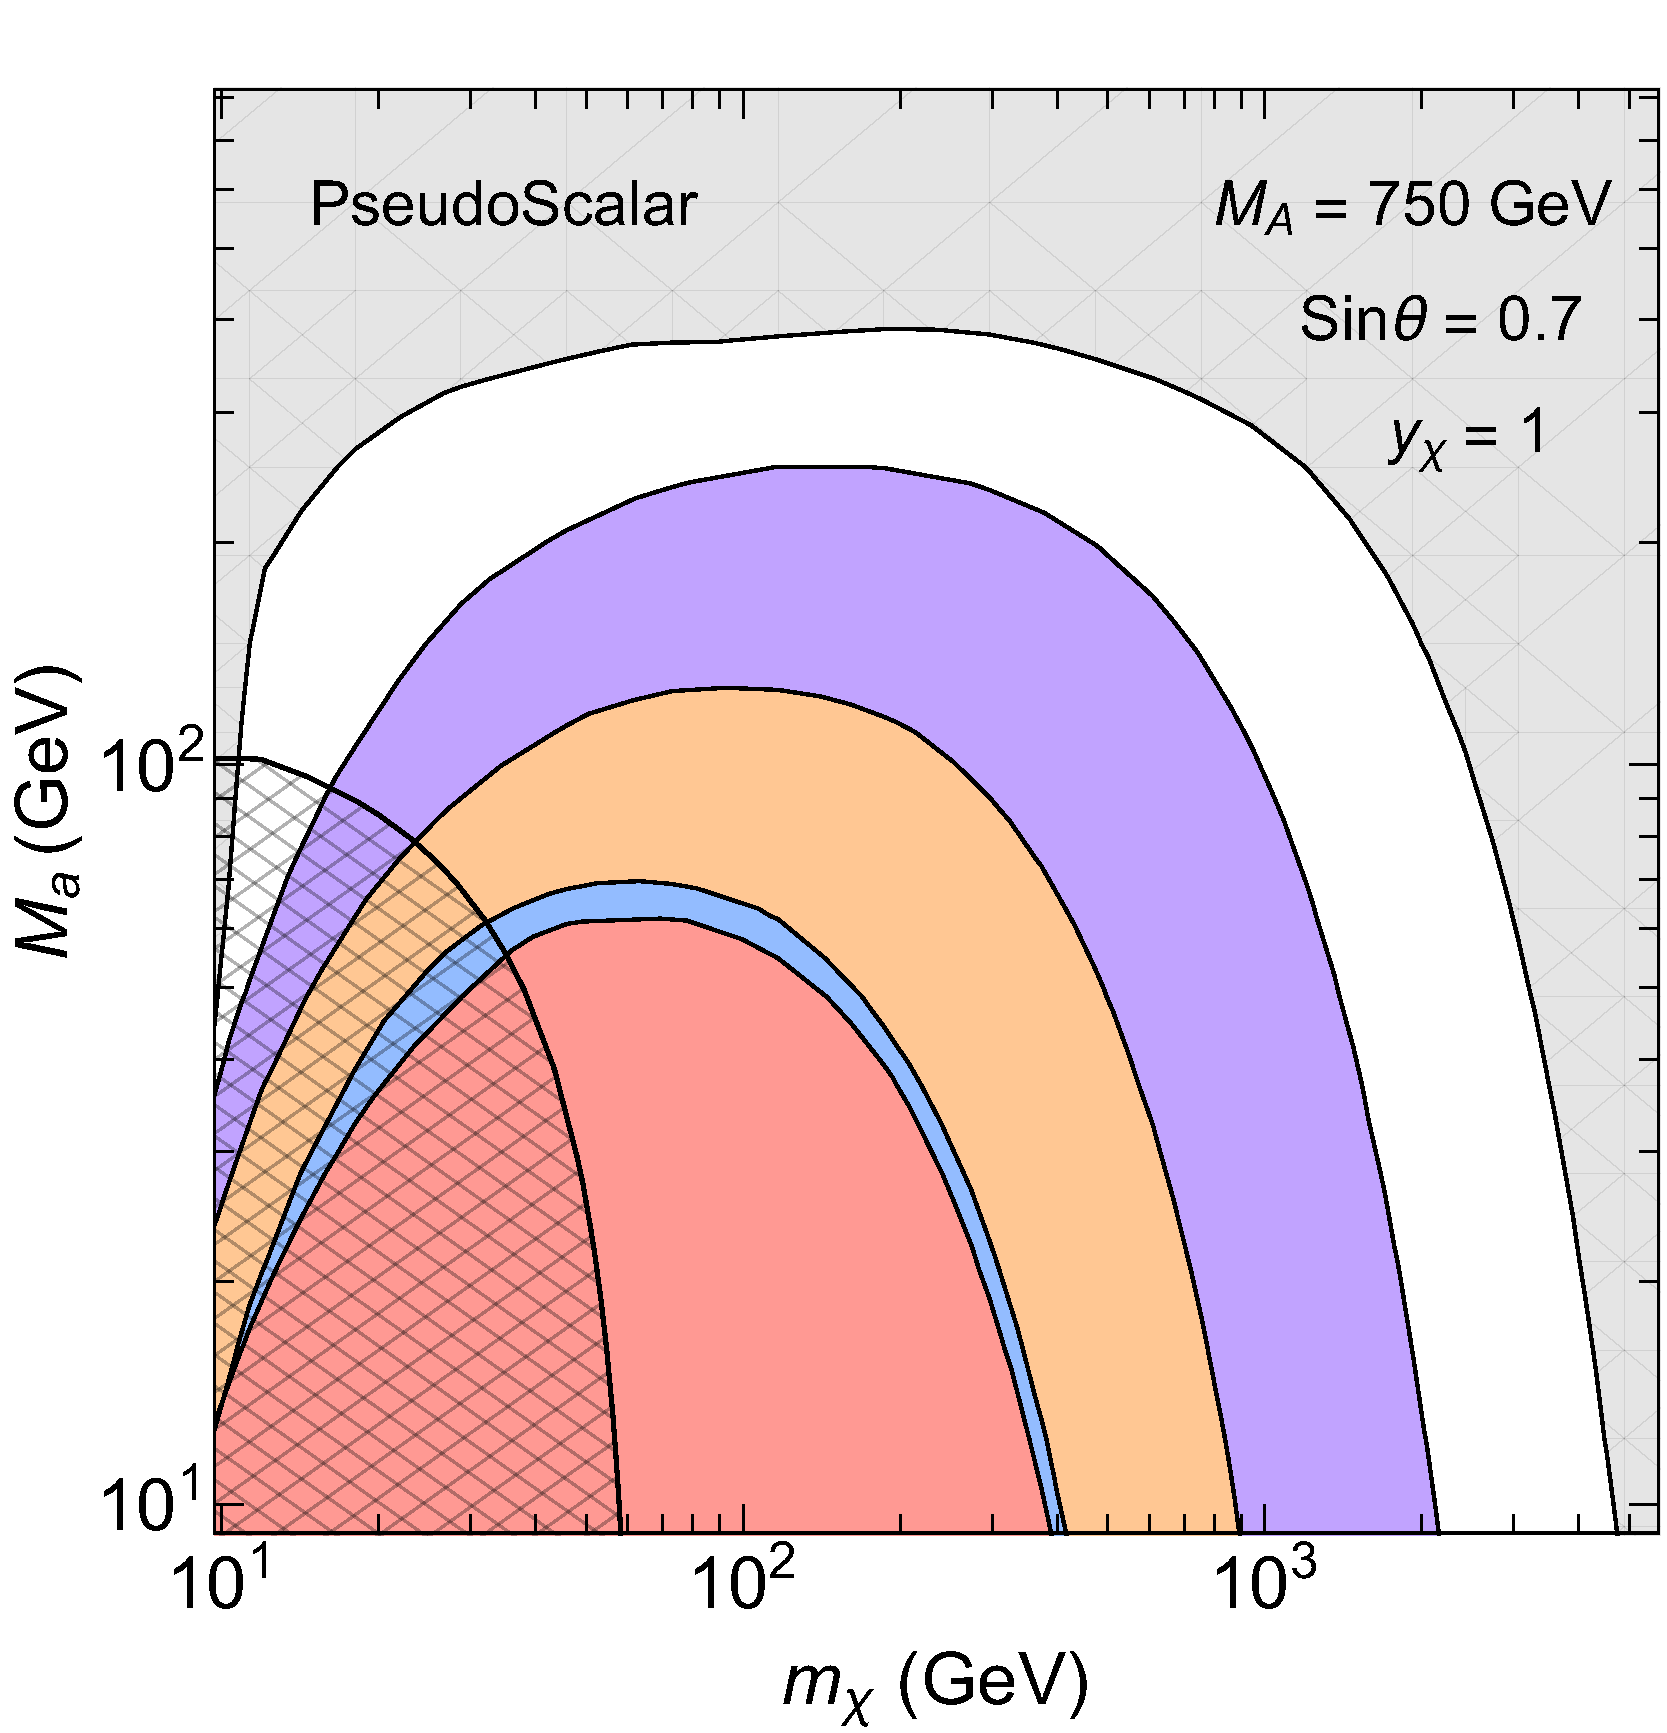
\includegraphics[width=0.49\textwidth]{texinputs/06_comparisons/figures/PseudoS07.pdf}
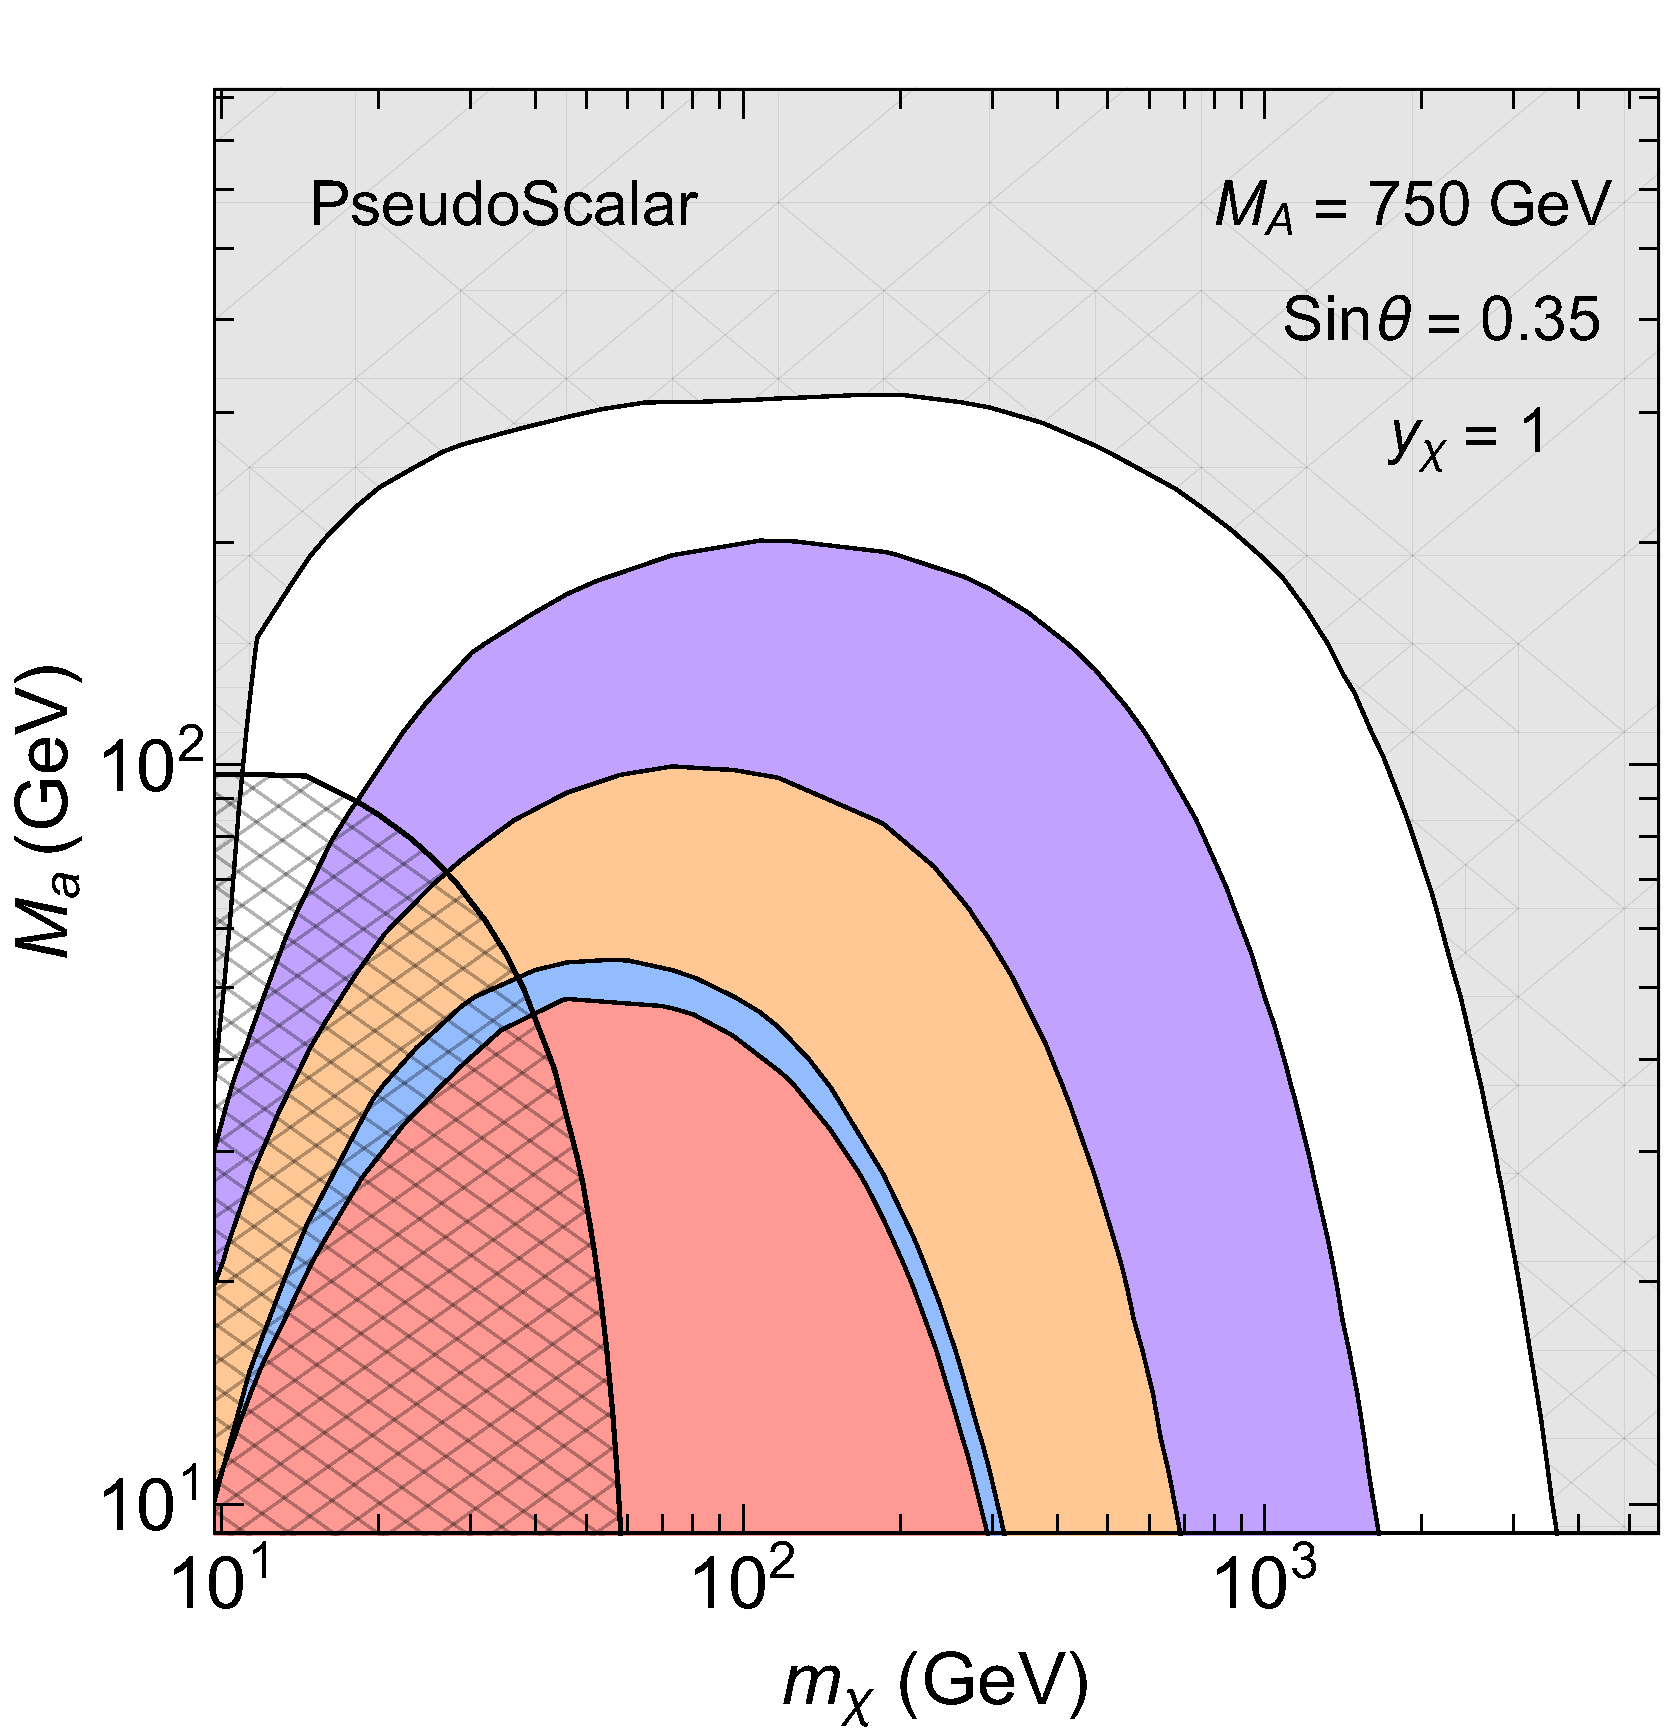
\includegraphics[width=0.49\textwidth]{texinputs/06_comparisons/figures/PseudoS035.pdf}\\
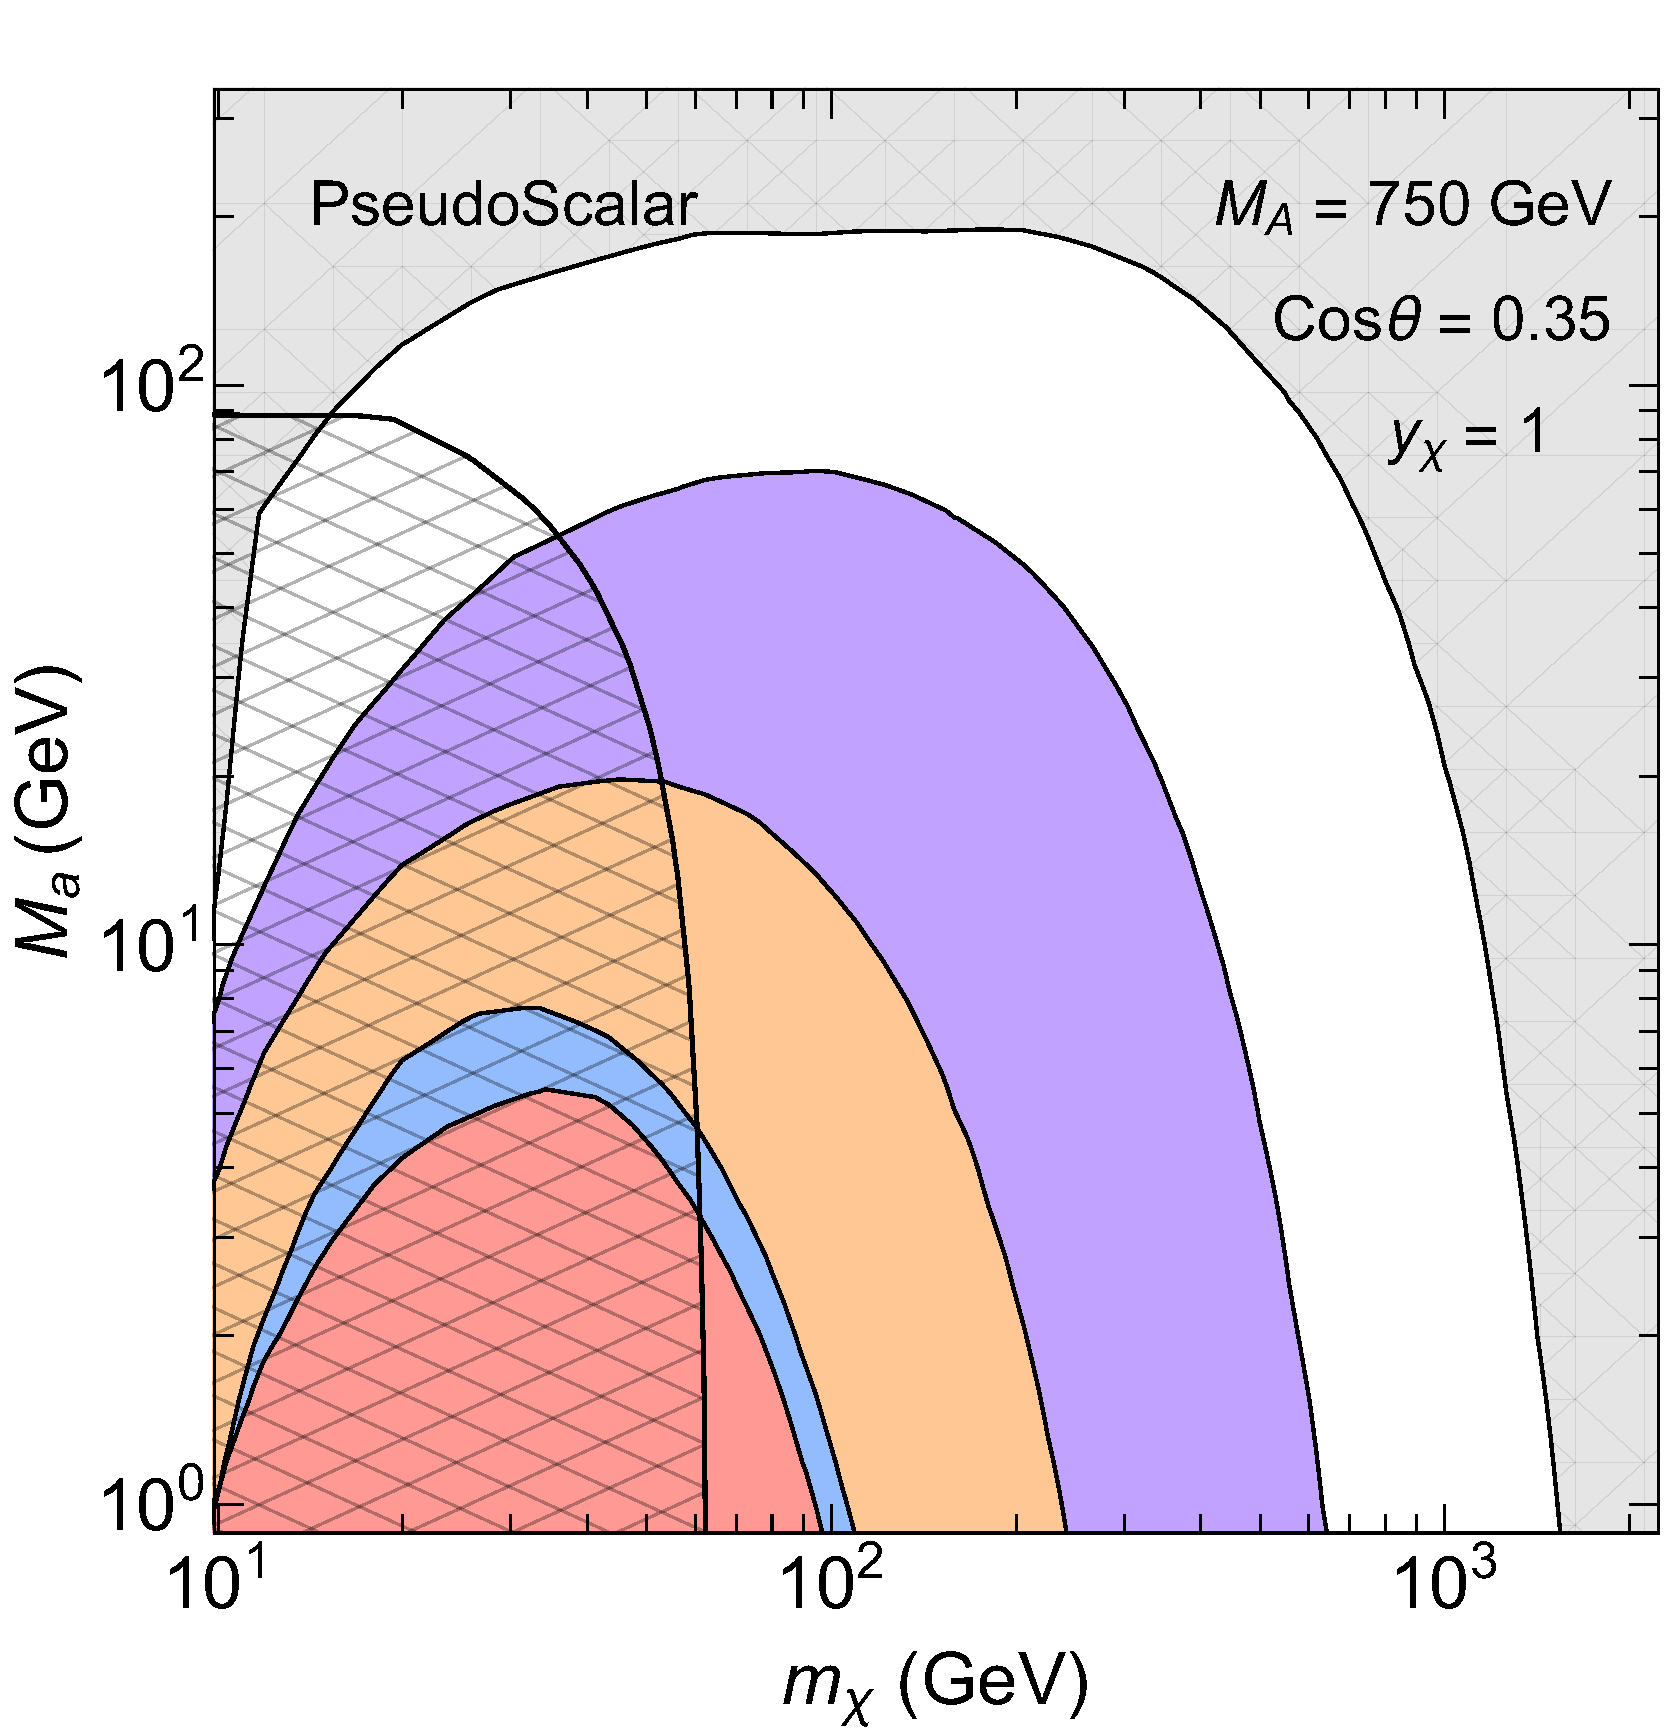
\includegraphics[width=0.49\textwidth]{texinputs/06_comparisons/figures/PseudoC035.pdf}
\caption{DD exclusion and projections for the first benchmark point for various experiments for the Pseudoscalar model. The various regions refer, in order, to LUX \citep{Akerib:2016vxi}, XENON1T\citep{Aprile:2017iyp}, XENON1T and XENONnT projections \citep{Aprile:2015uzo}, and neutrino background \citep{Billard:2013qya}. Top Left panel uses $\sin\theta=0.7$, top right panel uses $\cos\theta=0.35$, bottom panel uses $\cos\theta=0.35$, while $M_A=750\GeV$ in all the panels.} 
\label{fig:PSDD}
\end{center}
\end{figure} 


where the coefficients $\mu$ are given in terms of either the couplings in the $\Phi_{1,2}$ basis or in the $\Phi_{h,H}$ basis (indicated as $\hat{\mu}$), respectively:
\begin{eqnarray}
\mu_{AAh} &=& z\left(\cos^2\theta-\frac{2\lambda_3v^2}{m_h^2}\right), \label{eq:mu11h}\\
\mu_{Aah} &=& -\frac{1}{2}\sin(2\theta)\left(\frac{1}{x}-\frac{1}{y}+z\right),  \label{eq:mu12h}\\
\mu_{aah} &=& 2\sin^2(\theta)\left(\frac{1}{x}-\frac{1}{y}+\frac{z}{2}\right) -z\frac{2\lambda_3 v^2}{m_h^2},\label{eq:mu22h}\\
\hat{\mu}_{AAh} &=& -\frac{1}{2}\sin^2(2\theta)\left(\frac{1}{x}-\frac{1}{y}\right) - z\frac{\hat{\lambda}_{34-5}v^2}{m_h^2}\cos^2\theta -z\frac{2\hat{\lambda}_{P_1}v^2}{m_h^2}\sin^2\theta,  \label{eq:muAAh}\\
\hat{\mu}_{Aah} &=& -\frac{1}{4}\sin(4\theta)\left(\frac{1}{x}-\frac{1}{y}\right) + \frac{z}{2}\frac{(\hat{\lambda}_{345P}-2\hat{\lambda}_{P_1}) v^2}{m_h^2}\sin(2\theta), \label{eq:muaAh}\\
\hat{\mu}_{aah} &=& \frac{1}{2}\sin^2(2\theta)\left(\frac{1}{x}-\frac{1}{y}\right) -z\frac{\hat{\lambda}_{34-5}v^2}{m_h^2}\sin^2\theta +z\frac{2\hat{\lambda}_{P_1}v^2}{m_h^2}\cos^2\theta ,\label{eq:muaah}
\end{eqnarray}
The coefficient $\mu$ have been written under the assumption of alignment, and imposing $M_A=M_H=M_{H^+}$ and $\lambda_3=\lambda_{P_1}=\lambda_{P_2}$, while the coefficients $\hat{\mu}$ are using no assumption other than the alignment condition. The interference structure arising from gauge invariance is only manmisfest in the latter case.
Note that the terms proportional to $z$ arise from the terms in the 2HDM potential proportional to $\lambda_{1,2,3,4,5, P_1, P_2}$\footnote{Relations between $\hat{\lambda}_i$ and $\lambda_i$ can be found in \citep{Bell:2017rgi}.}, and in general their coefficient will depend on all these couplings and the value of $\tan\beta$. However, here we consider two example cases: the first one, where $\hat{\lambda}_{34-5}=\hat{\lambda}_3+\hat{\lambda}_4-\hat{\lambda}_5=\hat{\lambda}_1=\frac{m_h^2}{v^2}$ and $\hat{\lambda}_{P_1}=\hat{\lambda}_{P_2}=0$, and the second one with $\lambda_3=\lambda_{P_1}=\lambda_{P_2}=3$ and $\lambda_{4,5}$ set by the condition $M_H=M_A=M_{H^+}$. 

%The scattering of DM with nuclei will be dominated by the diagram shown in %Fig.\ref{fig:feynDDPS} for the pseudoscalar, resulting in a spin-independent %scattering cross section. The relevant nucleon operator is
%\begin{equation}
%O_1^N = \bar{\chi} \chi \bar{N} N,  \label{eq:op1}
%\end{equation}
%and, by integrating out the mediators, we obtain a coefficient of %\citep{Bell:2016ekl}
%\begin{equation}
%c_N^1 = m_N\frac{c_q}{m_q}\left(\sum_{q=u,d,s} f_{T_q}^N + \frac{2}{9} f_{T_g}  %\right).\label{eq:c1}
%\end{equation}

%The tree level scatterings are instead suppressed in both cases. For the %pseudoscalar, the relevant scattering operator is
%\begin{equation}
%O_4^N = \bar{\chi}\gamma^5 \chi \bar{N}\gamma^5 N,  \label{eq:op4}
%\end{equation}
%and it is spin-dependent and suppressed by $q_{tr}^4$. The coefficient of the %operator is
%\begin{equation}
%c_N^4 = m_N\frac{y_\chi %\cos\theta\sin\theta}{v}\left(\frac{1}{M_{S_1}^2}-\frac{1}{M_{S_2}^2}\right)\sum_{q=u,d,s} \left(\epsilon_q-\left(\epsilon_u+2\epsilon_d\right)\frac{\bar{m}}{m_q}\right)\Delta_q^{(N)}.\label{eq:c4}
%\end{equation}

\begin{figure}[ht]
\begin{center}
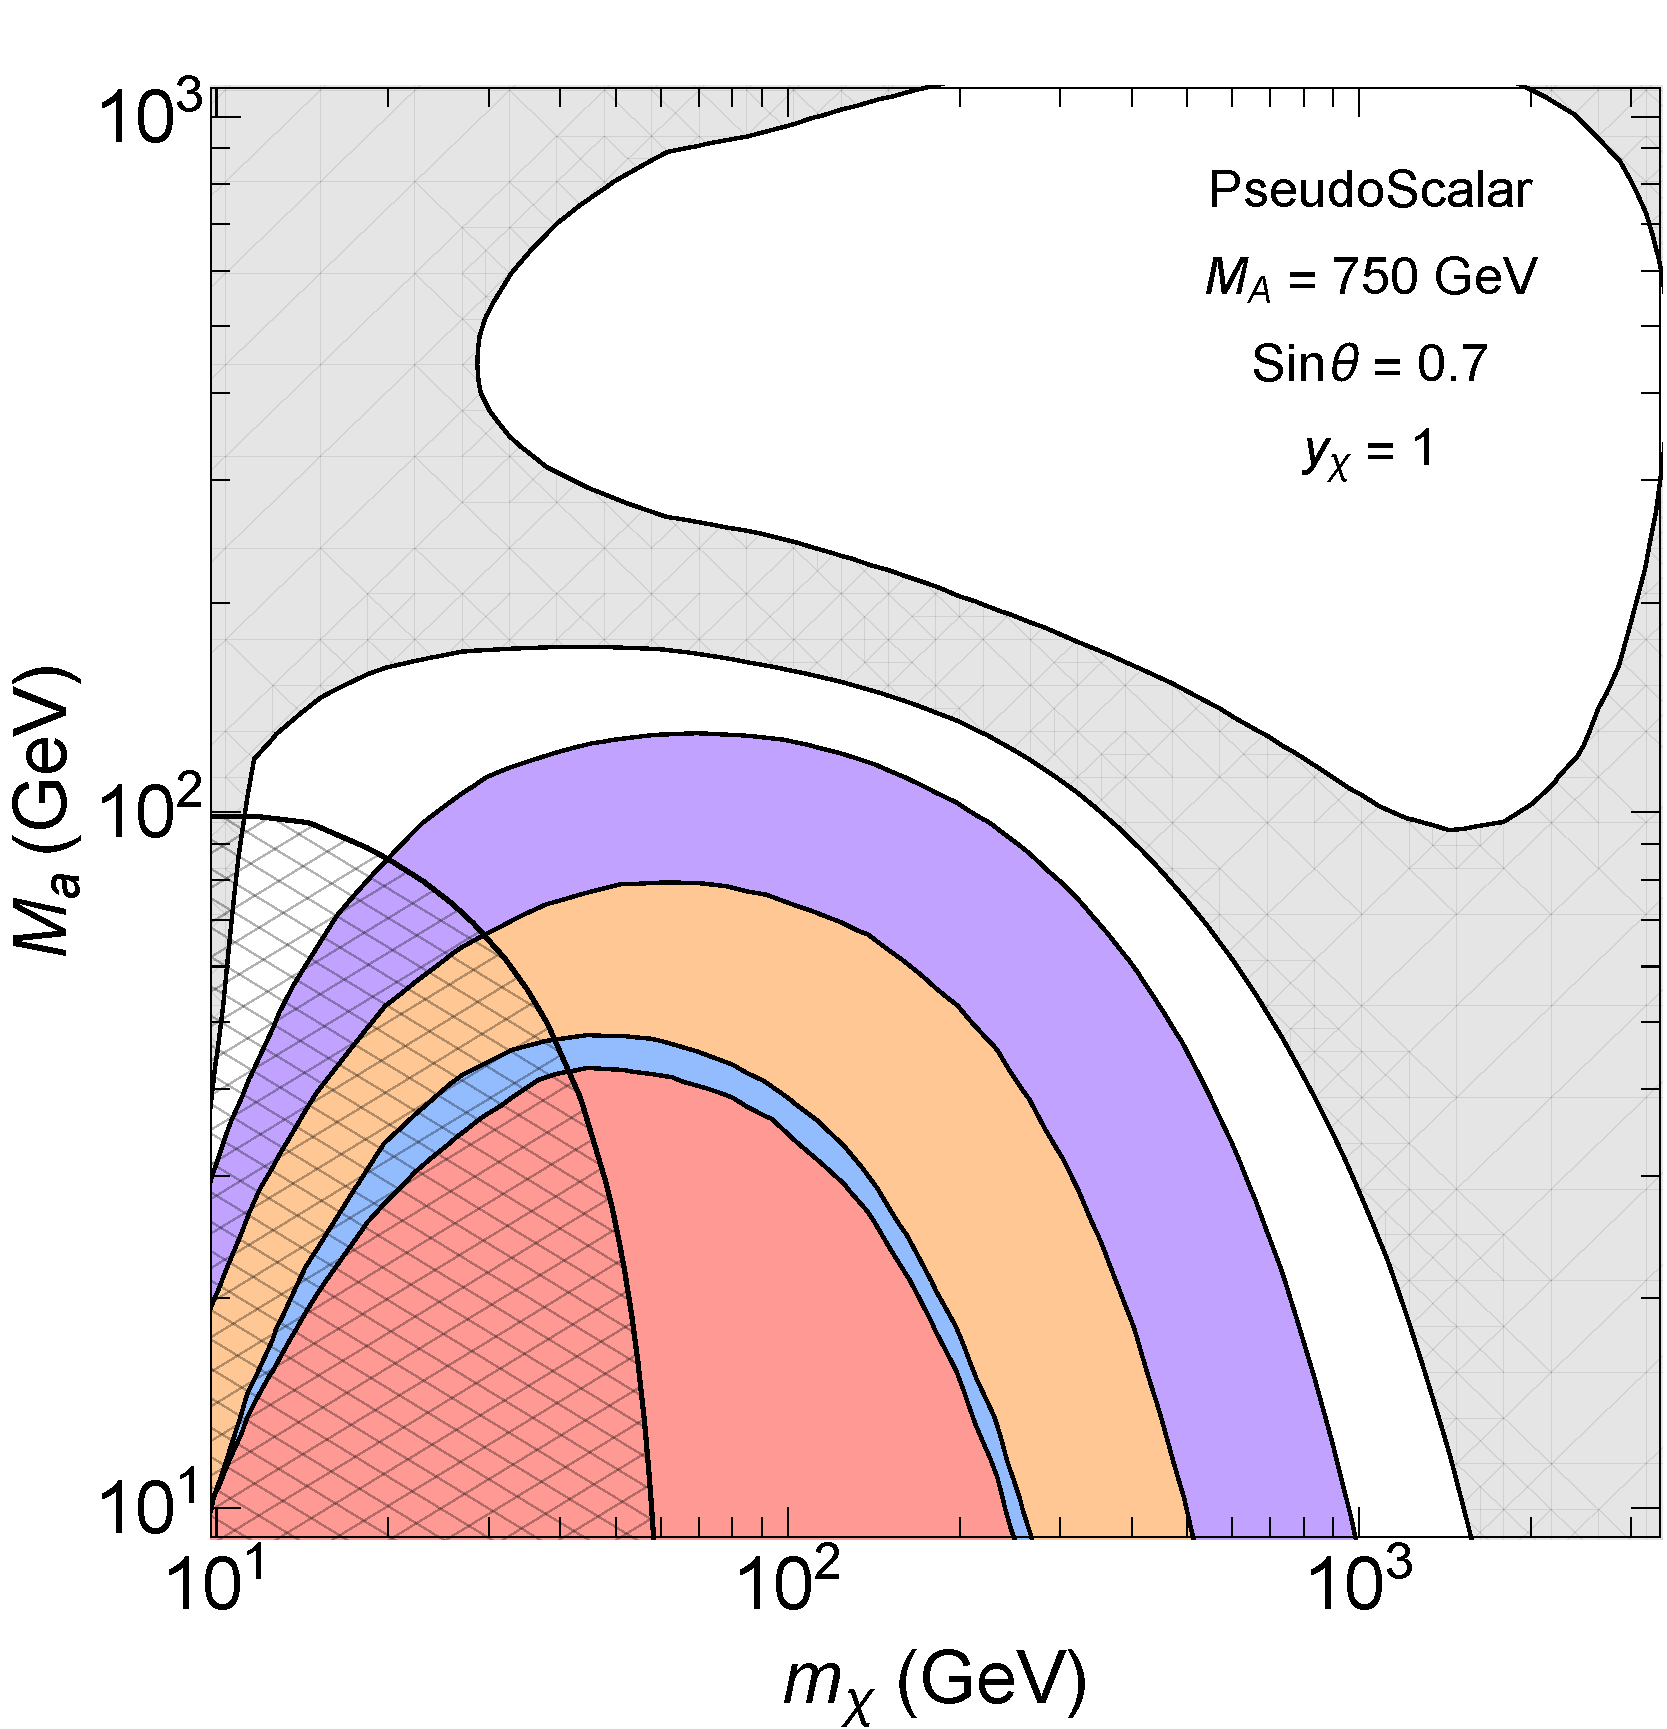
\includegraphics[width=0.49\textwidth]{texinputs/06_comparisons/figures/PS_F_S070.pdf}
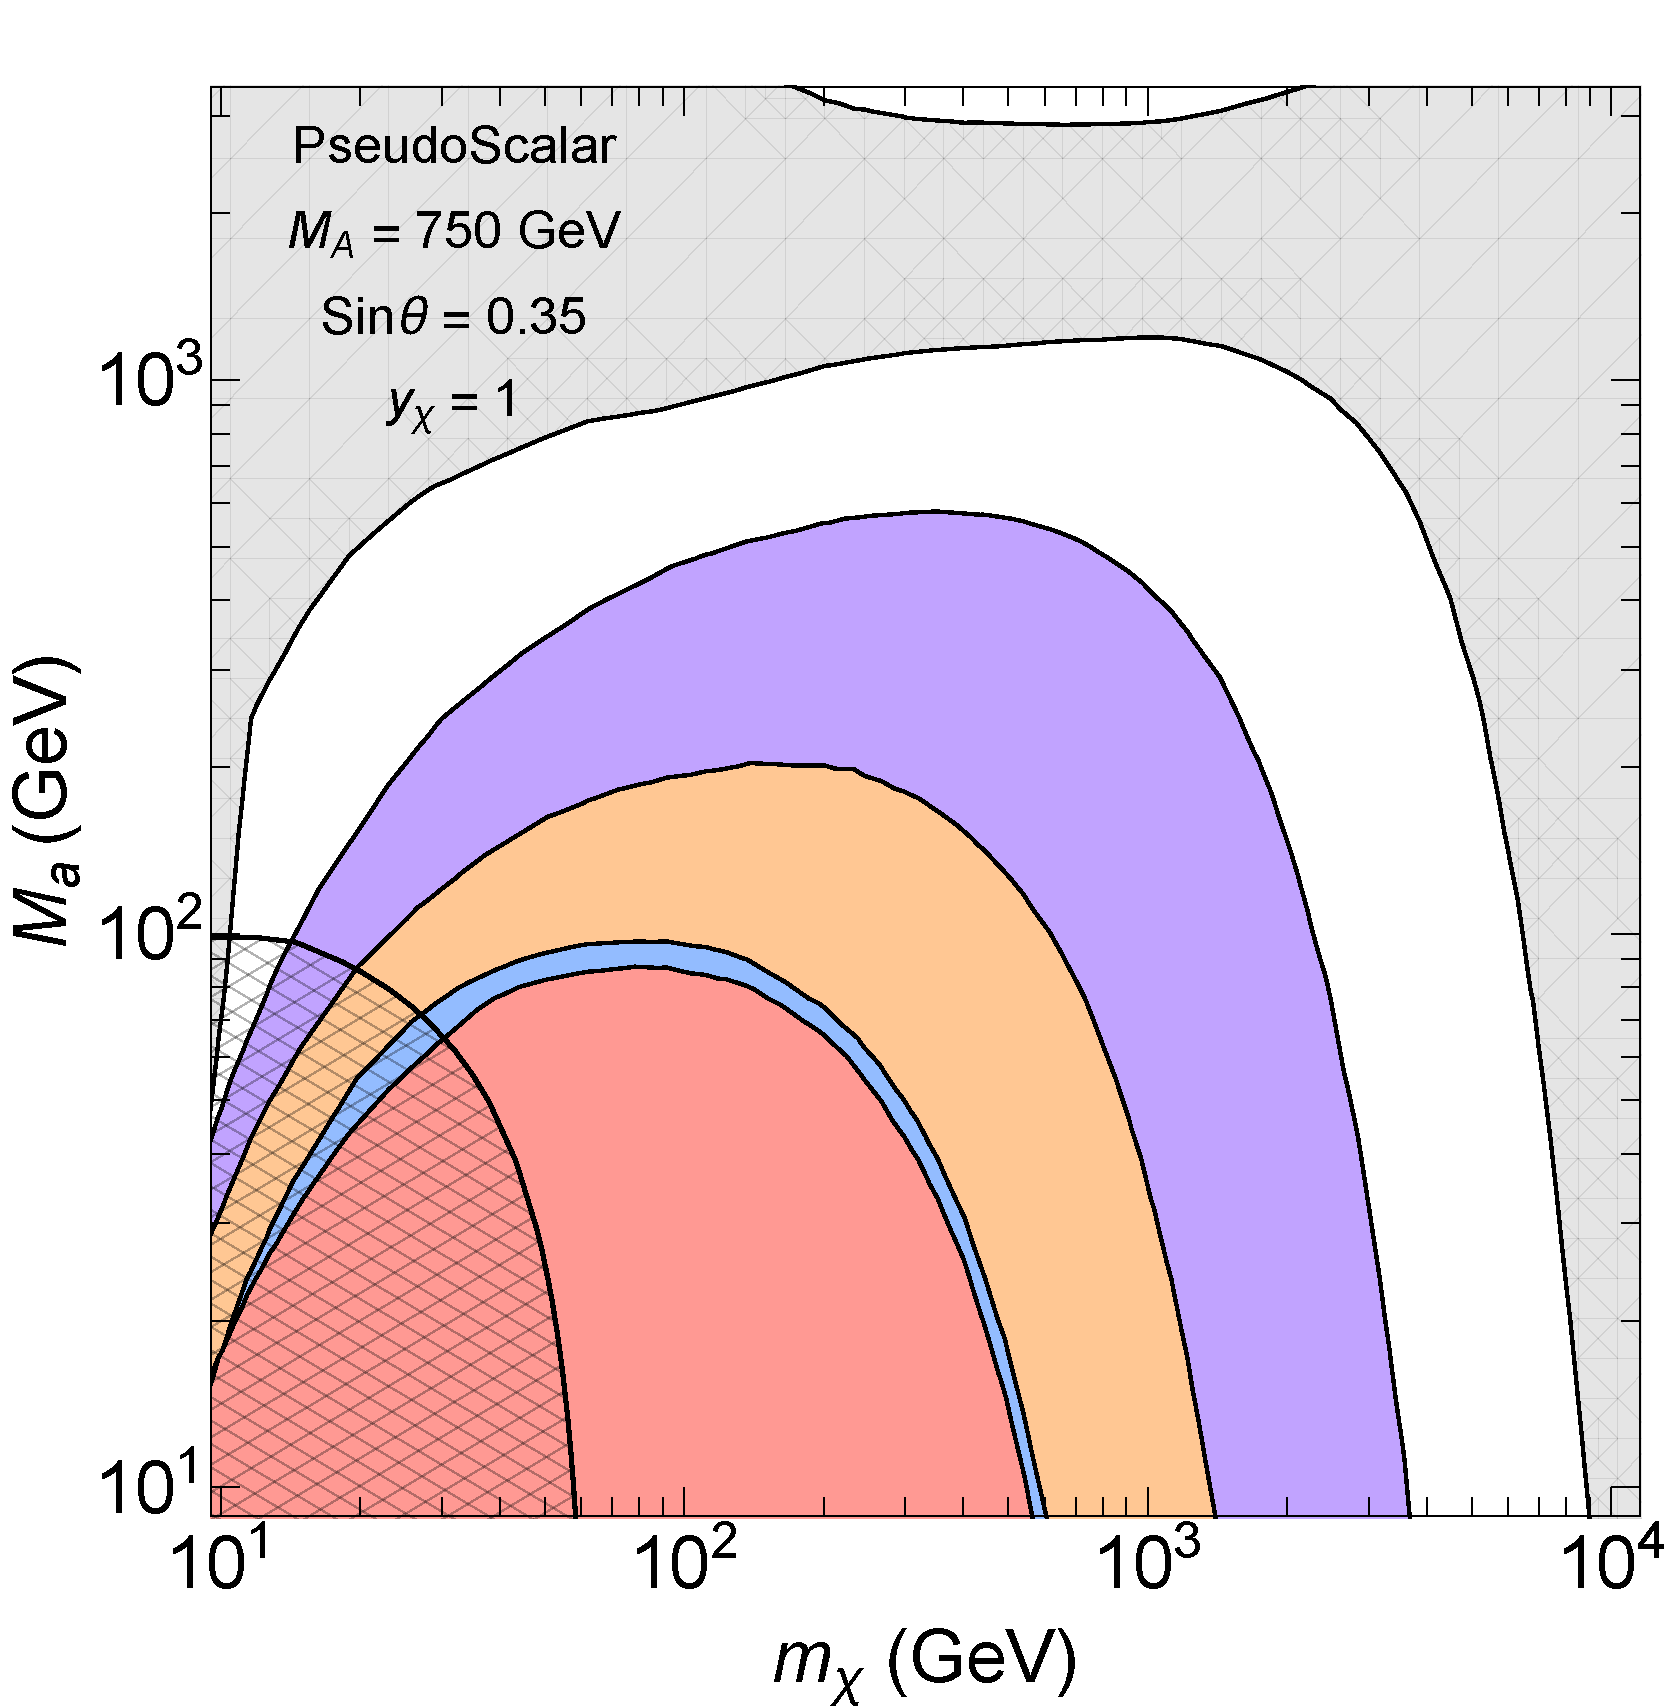
\includegraphics[width=0.49\textwidth]{texinputs/06_comparisons/figures/PS_F_S035.pdf}\\
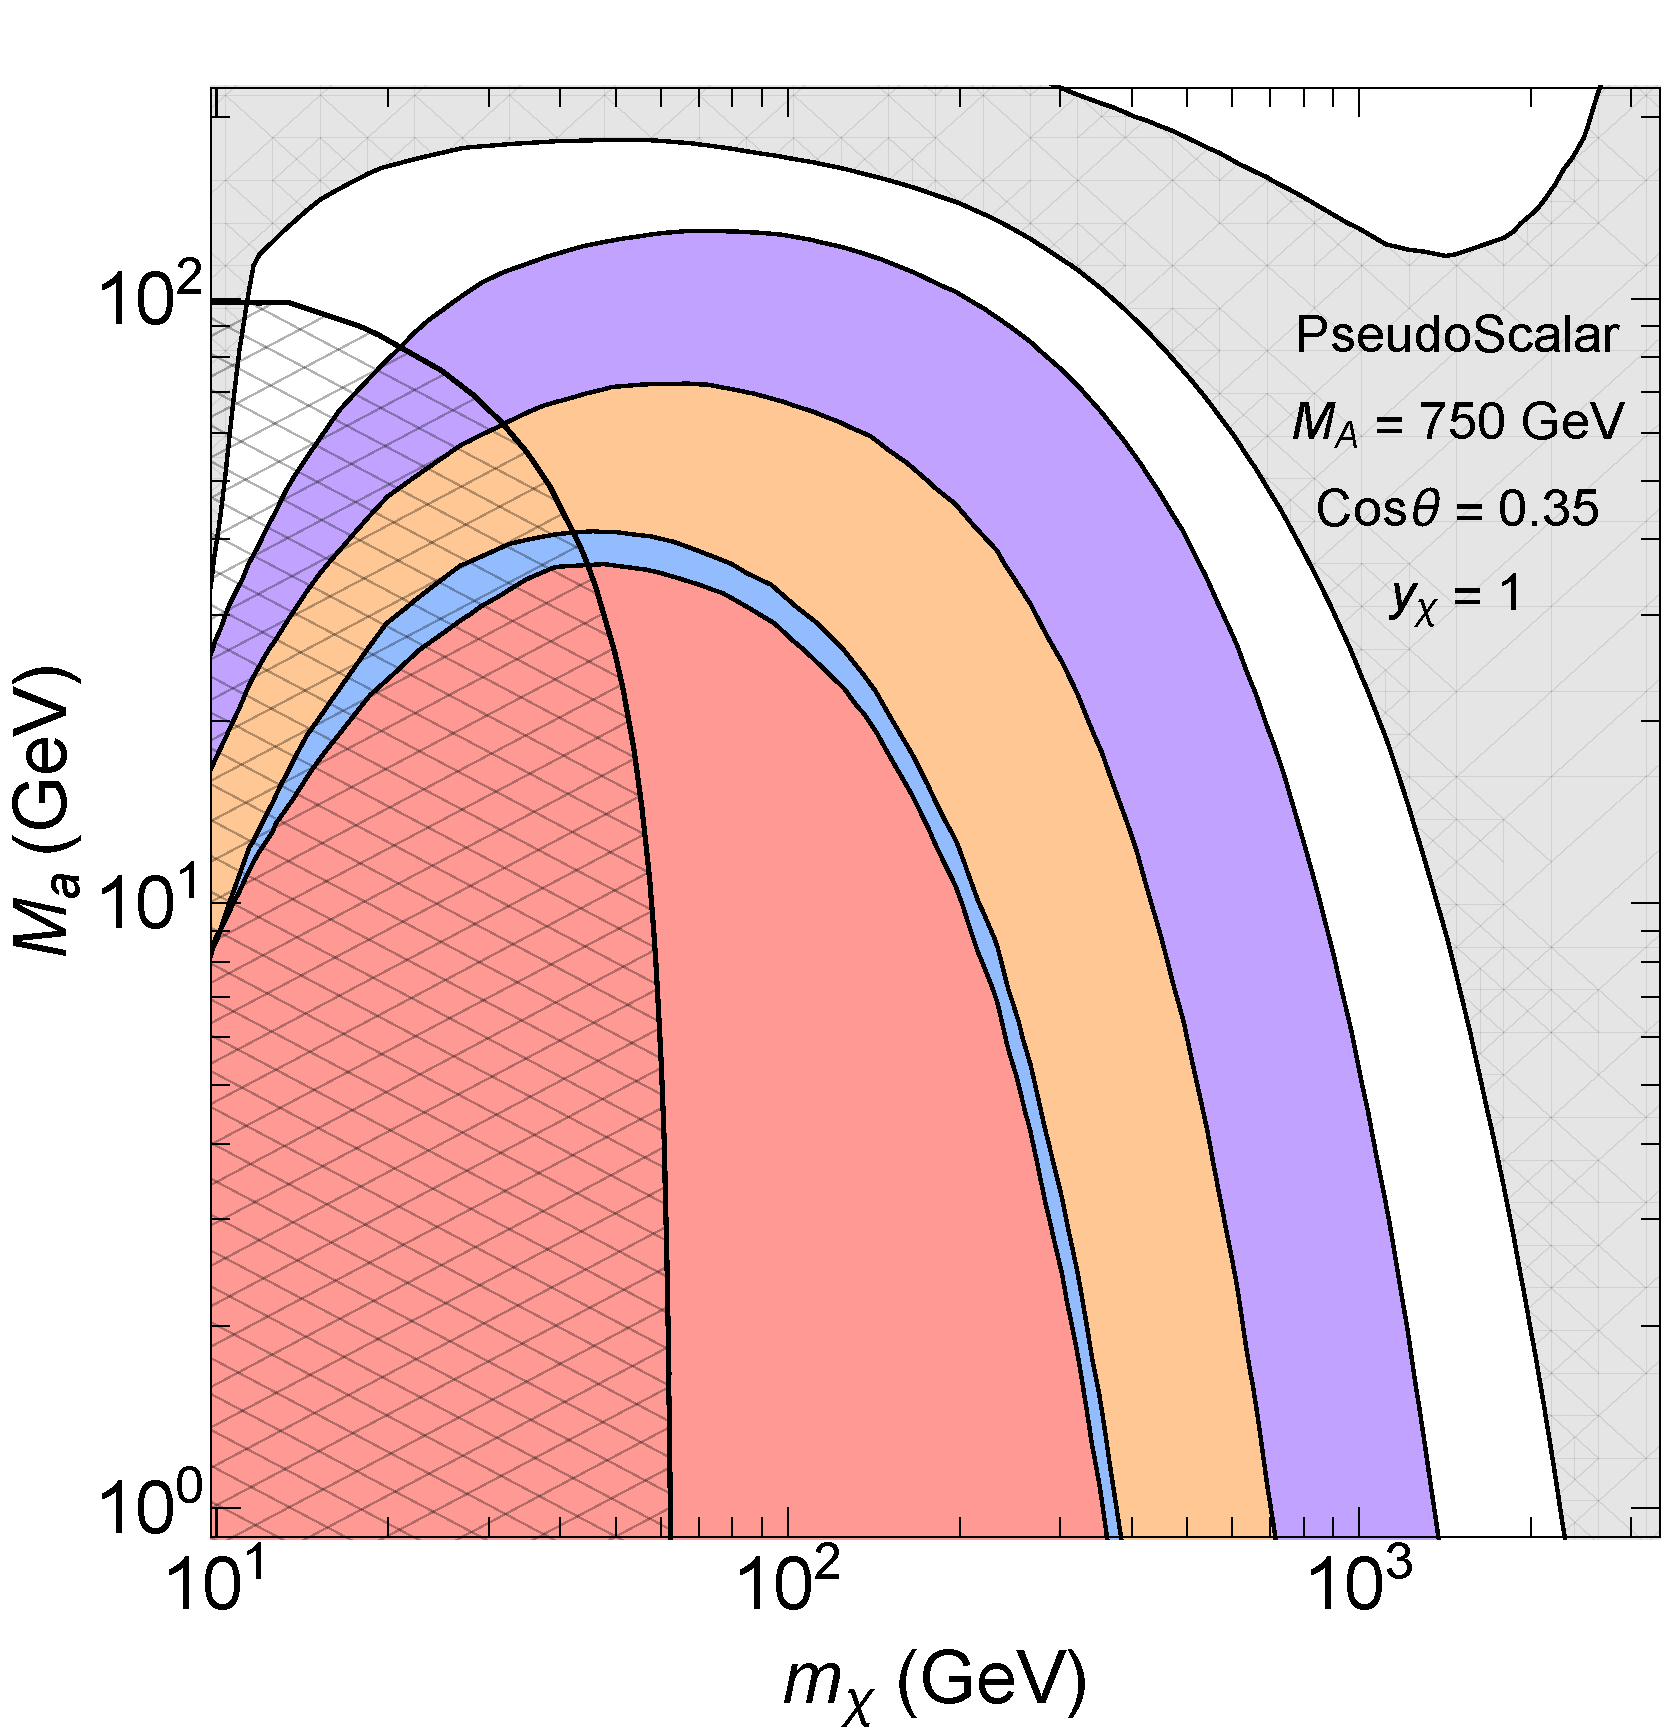
\includegraphics[width=0.49\textwidth]{texinputs/06_comparisons/figures/PS_F_C035.pdf}
\caption{DD exclusion and projections for the second benchmark point for the first benchmark point for various experiments for the Pseudoscalar model. The various regions refer, in order, to LUX \citep{Akerib:2016vxi}, XENON1T\citep{Aprile:2017iyp}, XENON1T and XENONnT projections \citep{Aprile:2015uzo}, and neutrino background \citep{Billard:2013qya}. Top Left panel uses $\sin\theta=0.7$, top right panel uses $\cos\theta=0.35$, bottom panel uses $\cos\theta=0.35$, while $M_A=750\GeV$ in all the panels.} 
\label{fig:PSDD2}
\end{center}
\end{figure} 

DD for the pseudoscalar model are presented in Fig. \ref{fig:PSDD} and \ref{fig:PSDD2} for the first and second benchmark point respectively. Limits are calculated using \ref{eq:loopps}. The heavier pseudoscalar is set to $M_A=750\GeV$, and the mixing angles are fixed to $\sin\theta=0.7$ in the left panel, $\sin\theta=0.35$ in the right panel and $\cos\theta=0.35$ in the bottom panel. In the first case, current limits are able to exclude the portion of parameter space with $20\GeV \lesssim m_\chi \lesssim 200\GeV$ and $M_a \lesssim 40\GeV$. Projected limits for XENON1T and XENONnT could expand the excluded region to $10\GeV \lesssim m_\chi \lesssim 1\TeV$ and $M_a \lesssim 150\GeV$. The presence of the neutrino floor will prevent to be able to probe this model for $M_a\gtrsim 300\GeV$ or $m_\chi \gtrsim 3\TeV$ with conventional DD experiments. The second case is quite similar to the first, with the limits just slightly weakened by the smaller mixing angle. In the last case, for $\cos\theta=0.35$, current DD experiments can only probe a tiny portion of the parameter space, with $20\GeV \lesssim m_\chi \lesssim 70\GeV$ and $M_a \lesssim 4\GeV$. We can see that indeed the whole region rules out by DD is contained in the region rules out by Higgs width constraints. Projected limits expand the range to up $M_a\sim 40\GeV$ and $m_\chi\sim 400\GeV$, while neutrino background makes inaccessible to DD the region beyond $M_A\gtrsim 100\GeV$ or $m_\chi \gtrsim 1\TeV$. In the 3 panels we also report limits from Higgs invisible BR \citep{Aad:2015pla,Khachatryan:2016whc}, coming from 2 and 3 body decays, as described in \citep{Bauer:2017ota}. They rule out the low $m_\chi,M_a$ mass region.
